\documentclass[1p]{elsarticle_modified}
%\bibliographystyle{elsarticle-num}

%\usepackage[colorlinks]{hyperref}
%\usepackage{abbrmath_seonhwa} %\Abb, \Ascr, \Acal ,\Abf, \Afrak
\usepackage{amsfonts}
\usepackage{amssymb}
\usepackage{amsmath}
\usepackage{amsthm}
\usepackage{scalefnt}
\usepackage{amsbsy}
\usepackage{kotex}
\usepackage{caption}
\usepackage{subfig}
\usepackage{color}
\usepackage{graphicx}
\usepackage{xcolor} %% white, black, red, green, blue, cyan, magenta, yellow
\usepackage{float}
\usepackage{setspace}
\usepackage{hyperref}

\usepackage{tikz}
\usetikzlibrary{arrows}

\usepackage{multirow}
\usepackage{array} % fixed length table
\usepackage{hhline}

%%%%%%%%%%%%%%%%%%%%%
\makeatletter
\renewcommand*\env@matrix[1][\arraystretch]{%
	\edef\arraystretch{#1}%
	\hskip -\arraycolsep
	\let\@ifnextchar\new@ifnextchar
	\array{*\c@MaxMatrixCols c}}
\makeatother %https://tex.stackexchange.com/questions/14071/how-can-i-increase-the-line-spacing-in-a-matrix
%%%%%%%%%%%%%%%

\usepackage[normalem]{ulem}

\newcommand{\msout}[1]{\ifmmode\text{\sout{\ensuremath{#1}}}\else\sout{#1}\fi}
%SOURCE: \msout is \stkout macro in https://tex.stackexchange.com/questions/20609/strikeout-in-math-mode

\newcommand{\cancel}[1]{
	\ifmmode
	{\color{red}\msout{#1}}
	\else
	{\color{red}\sout{#1}}
	\fi
}

\newcommand{\add}[1]{
	{\color{blue}\uwave{#1}}
}

\newcommand{\replace}[2]{
	\ifmmode
	{\color{red}\msout{#1}}{\color{blue}\uwave{#2}}
	\else
	{\color{red}\sout{#1}}{\color{blue}\uwave{#2}}
	\fi
}

\newcommand{\Sol}{\mathcal{S}} %segment
\newcommand{\D}{D} %diagram
\newcommand{\A}{\mathcal{A}} %arc


%%%%%%%%%%%%%%%%%%%%%%%%%%%%%5 test

\def\sl{\operatorname{\textup{SL}}(2,\Cbb)}
\def\psl{\operatorname{\textup{PSL}}(2,\Cbb)}
\def\quan{\mkern 1mu \triangleright \mkern 1mu}

\theoremstyle{definition}
\newtheorem{thm}{Theorem}[section]
\newtheorem{prop}[thm]{Proposition}
\newtheorem{lem}[thm]{Lemma}
\newtheorem{ques}[thm]{Question}
\newtheorem{cor}[thm]{Corollary}
\newtheorem{defn}[thm]{Definition}
\newtheorem{exam}[thm]{Example}
\newtheorem{rmk}[thm]{Remark}
\newtheorem{alg}[thm]{Algorithm}

\newcommand{\I}{\sqrt{-1}}
\begin{document}

%\begin{frontmatter}
%
%\title{Boundary parabolic representations of knots up to 8 crossings}
%
%%% Group authors per affiliation:
%\author{Yunhi Cho} 
%\address{Department of Mathematics, University of Seoul, Seoul, Korea}
%\ead{yhcho@uos.ac.kr}
%
%
%\author{Seonhwa Kim} %\fnref{s_kim}}
%\address{Center for Geometry and Physics, Institute for Basic Science, Pohang, 37673, Korea}
%\ead{ryeona17@ibs.re.kr}
%
%\author{Hyuk Kim}
%\address{Department of Mathematical Sciences, Seoul National University, Seoul 08826, Korea}
%\ead{hyukkim@snu.ac.kr}
%
%\author{Seokbeom Yoon}
%\address{Department of Mathematical Sciences, Seoul National University, Seoul, 08826,  Korea}
%\ead{sbyoon15@snu.ac.kr}
%
%\begin{abstract}
%We find all boundary parabolic representation of knots up to 8 crossings.
%
%\end{abstract}
%\begin{keyword}
%    \MSC[2010] 57M25 
%\end{keyword}
%
%\end{frontmatter}

%\linenumbers
%\tableofcontents
%
\newcommand\colored[1]{\textcolor{white}{\rule[-0.35ex]{0.8em}{1.4ex}}\kern-0.8em\color{red} #1}%
%\newcommand\colored[1]{\textcolor{white}{ #1}\kern-2.17ex	\textcolor{white}{ #1}\kern-1.81ex	\textcolor{white}{ #1}\kern-2.15ex\color{red}#1	}

{\Large $\underline{12a_{1252}~(K12a_{1252})}$}

\setlength{\tabcolsep}{10pt}
\renewcommand{\arraystretch}{1.6}
\vspace{1cm}\begin{tabular}{m{100pt}>{\centering\arraybackslash}m{274pt}}
\multirow{5}{120pt}{
	\centering
	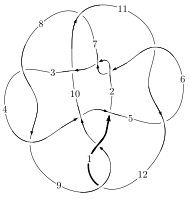
\includegraphics[width=112pt]{../../../GIT/diagram.site/Diagrams/png/2053_12a_1252.png}\\
\ \ \ A knot diagram\footnotemark}&
\allowdisplaybreaks
\textbf{Linearized knot diagam} \\
\cline{2-2}
 &
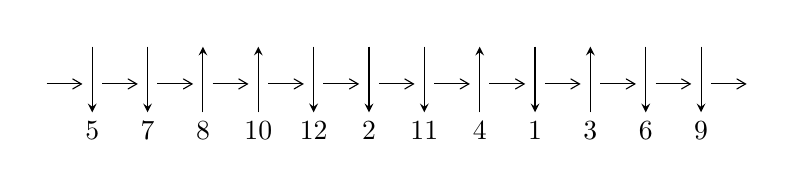
\begin{tikzpicture}[x=20pt, y=17pt]
	% nodes
	\node (C0) at (0, 0) {};
	\node (C1) at (1, 0) {};
	\node (C1U) at (1, +1) {};
	\node (C1D) at (1, -1) {5};

	\node (C2) at (2, 0) {};
	\node (C2U) at (2, +1) {};
	\node (C2D) at (2, -1) {7};

	\node (C3) at (3, 0) {};
	\node (C3U) at (3, +1) {};
	\node (C3D) at (3, -1) {8};

	\node (C4) at (4, 0) {};
	\node (C4U) at (4, +1) {};
	\node (C4D) at (4, -1) {10};

	\node (C5) at (5, 0) {};
	\node (C5U) at (5, +1) {};
	\node (C5D) at (5, -1) {12};

	\node (C6) at (6, 0) {};
	\node (C6U) at (6, +1) {};
	\node (C6D) at (6, -1) {2};

	\node (C7) at (7, 0) {};
	\node (C7U) at (7, +1) {};
	\node (C7D) at (7, -1) {11};

	\node (C8) at (8, 0) {};
	\node (C8U) at (8, +1) {};
	\node (C8D) at (8, -1) {4};

	\node (C9) at (9, 0) {};
	\node (C9U) at (9, +1) {};
	\node (C9D) at (9, -1) {1};

	\node (C10) at (10, 0) {};
	\node (C10U) at (10, +1) {};
	\node (C10D) at (10, -1) {3};

	\node (C11) at (11, 0) {};
	\node (C11U) at (11, +1) {};
	\node (C11D) at (11, -1) {6};

	\node (C12) at (12, 0) {};
	\node (C12U) at (12, +1) {};
	\node (C12D) at (12, -1) {9};
	\node (C13) at (13, 0) {};

	% arrows
	\draw[->,>={angle 60}]
	(C0) edge (C1) (C1) edge (C2) (C2) edge (C3) (C3) edge (C4) (C4) edge (C5) (C5) edge (C6) (C6) edge (C7) (C7) edge (C8) (C8) edge (C9) (C9) edge (C10) (C10) edge (C11) (C11) edge (C12) (C12) edge (C13) ;	\draw[->,>=stealth]
	(C1U) edge (C1D) (C2U) edge (C2D) (C3D) edge (C3U) (C4D) edge (C4U) (C5U) edge (C5D) (C6U) edge (C6D) (C7U) edge (C7D) (C8D) edge (C8U) (C9U) edge (C9D) (C10D) edge (C10U) (C11U) edge (C11D) (C12U) edge (C12D) ;
	\end{tikzpicture} \\
\hhline{~~} \\& 
\textbf{Solving Sequence} \\ \cline{2-2} 
 &
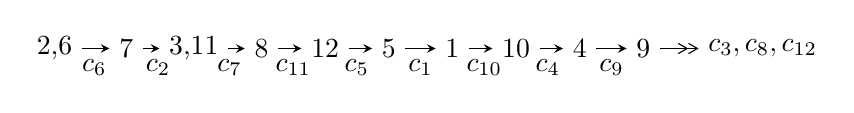
\begin{tikzpicture}[x=23pt, y=7pt]
	% node
	\node (A0) at (-1/8, 0) {2,6};
	\node (A1) at (1, 0) {7};
	\node (A2) at (33/16, 0) {3,11};
	\node (A3) at (25/8, 0) {8};
	\node (A4) at (33/8, 0) {12};
	\node (A5) at (41/8, 0) {5};
	\node (A6) at (49/8, 0) {1};
	\node (A7) at (57/8, 0) {10};
	\node (A8) at (65/8, 0) {4};
	\node (A9) at (73/8, 0) {9};
	\node (C1) at (1/2, -1) {$c_{6}$};
	\node (C2) at (3/2, -1) {$c_{2}$};
	\node (C3) at (21/8, -1) {$c_{7}$};
	\node (C4) at (29/8, -1) {$c_{11}$};
	\node (C5) at (37/8, -1) {$c_{5}$};
	\node (C6) at (45/8, -1) {$c_{1}$};
	\node (C7) at (53/8, -1) {$c_{10}$};
	\node (C8) at (61/8, -1) {$c_{4}$};
	\node (C9) at (69/8, -1) {$c_{9}$};
	\node (A10) at (11, 0) {$c_{3},c_{8},c_{12}$};

	% edge
	\draw[->,>=stealth]	
	(A0) edge (A1) (A1) edge (A2) (A2) edge (A3) (A3) edge (A4) (A4) edge (A5) (A5) edge (A6) (A6) edge (A7) (A7) edge (A8) (A8) edge (A9) ;
	\draw[->>,>={angle 60}]	
	(A9) edge (A10);
\end{tikzpicture} \\ 

\end{tabular} \\

\footnotetext{
The image of knot diagram is generated by the software ``\textbf{Draw programme}" developed by Andrew Bartholomew(\url{http://www.layer8.co.uk/maths/draw/index.htm\#Running-draw}), where we modified some parts for our purpose(\url{https://github.com/CATsTAILs/LinksPainter}).
}\phantom \\ \newline 
\centering \textbf{Ideals for irreducible components\footnotemark of $X_{\text{par}}$} 
 
\begin{align*}
I^u_{1}&=\langle 
1.05887\times10^{810} u^{147}-2.27511\times10^{810} u^{146}+\cdots+8.89868\times10^{809} b+7.85959\times10^{811},\\
\phantom{I^u_{1}}&\phantom{= \langle  }4.95430\times10^{810} u^{147}-1.09395\times10^{811} u^{146}+\cdots+7.11894\times10^{810} a+2.23800\times10^{812},\\
\phantom{I^u_{1}}&\phantom{= \langle  }u^{148}-3 u^{147}+\cdots+1664 u-64\rangle \\
I^u_{2}&=\langle 
-3.69653\times10^{27} u^{31}+1.94930\times10^{27} u^{30}+\cdots+1.18072\times10^{28} b+3.70363\times10^{28},\\
\phantom{I^u_{2}}&\phantom{= \langle  }1.05394\times10^{28} u^{31}-9.29787\times10^{27} u^{30}+\cdots+1.18072\times10^{28} a-1.82165\times10^{29},\;u^{32}- u^{31}+\cdots-32 u+4\rangle \\
I^u_{3}&=\langle 
b+1,\;a+2,\;u+1\rangle \\
\\
\end{align*}
\raggedright * 3 irreducible components of $\dim_{\mathbb{C}}=0$, with total 181 representations.\\
\footnotetext{All coefficients of polynomials are rational numbers. But the coefficients are sometimes approximated in decimal forms when there is not enough margin.}
\newpage
\renewcommand{\arraystretch}{1}
\centering \section*{I. $I^u_{1}= \langle 1.06\times10^{810} u^{147}-2.28\times10^{810} u^{146}+\cdots+8.90\times10^{809} b+7.86\times10^{811},\;4.95\times10^{810} u^{147}-1.09\times10^{811} u^{146}+\cdots+7.12\times10^{810} a+2.24\times10^{812},\;u^{148}-3 u^{147}+\cdots+1664 u-64 \rangle$}
\flushleft \textbf{(i) Arc colorings}\\
\begin{tabular}{m{7pt} m{180pt} m{7pt} m{180pt} }
\flushright $a_{2}=$&$\begin{pmatrix}0\\u\end{pmatrix}$ \\
\flushright $a_{6}=$&$\begin{pmatrix}1\\0\end{pmatrix}$ \\
\flushright $a_{7}=$&$\begin{pmatrix}1\\u^2\end{pmatrix}$ \\
\flushright $a_{3}=$&$\begin{pmatrix}- u\\- u^3+u\end{pmatrix}$ \\
\flushright $a_{11}=$&$\begin{pmatrix}-0.695932 u^{147}+1.53668 u^{146}+\cdots+1076.78 u-31.4373\\-1.18992 u^{147}+2.55668 u^{146}+\cdots+2177.36 u-88.3231\end{pmatrix}$ \\
\flushright $a_{8}=$&$\begin{pmatrix}0.858311 u^{147}-1.88226 u^{146}+\cdots-1494.64 u+53.2154\\-0.532878 u^{147}+1.17822 u^{146}+\cdots+1069.01 u-42.7677\end{pmatrix}$ \\
\flushright $a_{12}=$&$\begin{pmatrix}0.493986 u^{147}-1.02000 u^{146}+\cdots-1100.58 u+56.8858\\-1.18992 u^{147}+2.55668 u^{146}+\cdots+2177.36 u-88.3231\end{pmatrix}$ \\
\flushright $a_{5}=$&$\begin{pmatrix}-0.625260 u^{147}+1.36525 u^{146}+\cdots+1031.38 u-32.9940\\-0.0734242 u^{147}+0.157657 u^{146}+\cdots-160.009 u+6.08635\end{pmatrix}$ \\
\flushright $a_{1}=$&$\begin{pmatrix}0.906475 u^{147}-1.94690 u^{146}+\cdots-1819.41 u+78.0628\\-1.02336 u^{147}+2.25345 u^{146}+\cdots+1988.38 u-80.5304\end{pmatrix}$ \\
\flushright $a_{10}=$&$\begin{pmatrix}0.345697 u^{147}-0.716800 u^{146}+\cdots-861.448 u+46.6551\\-1.48200 u^{147}+3.18936 u^{146}+\cdots+2732.24 u-110.645\end{pmatrix}$ \\
\flushright $a_{4}=$&$\begin{pmatrix}-1.01014 u^{147}+2.19116 u^{146}+\cdots+1778.97 u-69.2538\\0.887000 u^{147}-1.95334 u^{146}+\cdots-1752.90 u+70.5881\end{pmatrix}$ \\
\flushright $a_{9}=$&$\begin{pmatrix}0.601293 u^{147}-1.26852 u^{146}+\cdots-1162.24 u+53.7405\\-0.984196 u^{147}+2.14628 u^{146}+\cdots+1887.69 u-76.4534\end{pmatrix}$\\&\end{tabular}
\flushleft \textbf{(ii) Obstruction class $= -1$}\\~\\
\flushleft \textbf{(iii) Cusp Shapes $= -2.98535 u^{147}+4.27263 u^{146}+\cdots+9435.88 u-379.745$}\\~\\
\newpage\renewcommand{\arraystretch}{1}
\flushleft \textbf{(iv) u-Polynomials at the component}\newline \\
\begin{tabular}{m{50pt}|m{274pt}}
Crossings & \hspace{64pt}u-Polynomials at each crossing \\
\hline $$\begin{aligned}c_{1}\end{aligned}$$&$\begin{aligned}
&u^{148}+7 u^{147}+\cdots+309248 u-8192
\end{aligned}$\\
\hline $$\begin{aligned}c_{2},c_{6}\end{aligned}$$&$\begin{aligned}
&u^{148}-3 u^{147}+\cdots+1664 u-64
\end{aligned}$\\
\hline $$\begin{aligned}c_{3},c_{8}\end{aligned}$$&$\begin{aligned}
&u^{148}-53 u^{146}+\cdots-69528 u-5398
\end{aligned}$\\
\hline $$\begin{aligned}c_{4}\end{aligned}$$&$\begin{aligned}
&u^{148}+12 u^{147}+\cdots+890247 u+39209
\end{aligned}$\\
\hline $$\begin{aligned}c_{5},c_{11}\end{aligned}$$&$\begin{aligned}
&u^{148}+12 u^{147}+\cdots-190801 u+15047
\end{aligned}$\\
\hline $$\begin{aligned}c_{7}\end{aligned}$$&$\begin{aligned}
&u^{148}+8 u^{147}+\cdots-1488 u+352
\end{aligned}$\\
\hline $$\begin{aligned}c_{9},c_{12}\end{aligned}$$&$\begin{aligned}
&u^{148}-2 u^{147}+\cdots+5011 u+1511
\end{aligned}$\\
\hline $$\begin{aligned}c_{10}\end{aligned}$$&$\begin{aligned}
&u^{148}+8 u^{147}+\cdots+92 u-8
\end{aligned}$\\
\hline
\end{tabular}\\~\\
\newpage\renewcommand{\arraystretch}{1}
\flushleft \textbf{(v) Riley Polynomials at the component}\newline \\
\begin{tabular}{m{50pt}|m{274pt}}
Crossings & \hspace{64pt}Riley Polynomials at each crossing \\
\hline $$\begin{aligned}c_{1}\end{aligned}$$&$\begin{aligned}
&y^{148}-29 y^{147}+\cdots-82061557760 y+67108864
\end{aligned}$\\
\hline $$\begin{aligned}c_{2},c_{6}\end{aligned}$$&$\begin{aligned}
&y^{148}-97 y^{147}+\cdots-472064 y+4096
\end{aligned}$\\
\hline $$\begin{aligned}c_{3},c_{8}\end{aligned}$$&$\begin{aligned}
&y^{148}-106 y^{147}+\cdots-7039344540 y+29138404
\end{aligned}$\\
\hline $$\begin{aligned}c_{4}\end{aligned}$$&$\begin{aligned}
&y^{148}-86 y^{147}+\cdots-56591966597 y+1537345681
\end{aligned}$\\
\hline $$\begin{aligned}c_{5},c_{11}\end{aligned}$$&$\begin{aligned}
&y^{148}-6 y^{147}+\cdots-1680126787 y+226412209
\end{aligned}$\\
\hline $$\begin{aligned}c_{7}\end{aligned}$$&$\begin{aligned}
&y^{148}+26 y^{147}+\cdots+1328384 y+123904
\end{aligned}$\\
\hline $$\begin{aligned}c_{9},c_{12}\end{aligned}$$&$\begin{aligned}
&y^{148}-74 y^{147}+\cdots-53825165 y+2283121
\end{aligned}$\\
\hline $$\begin{aligned}c_{10}\end{aligned}$$&$\begin{aligned}
&y^{148}-92 y^{147}+\cdots-7376 y+64
\end{aligned}$\\
\hline
\end{tabular}\\~\\
\newpage\flushleft \textbf{(vi) Complex Volumes and Cusp Shapes}
$$\begin{array}{c|c|c}  
\text{Solutions to }I^u_{1}& \I (\text{vol} + \sqrt{-1}CS) & \text{Cusp shape}\\
 \hline 
\begin{aligned}
u &= -0.998975\phantom{ +0.000000I} \\
a &= -9.00379\phantom{ +0.000000I} \\
b &= -8.88000\phantom{ +0.000000I}\end{aligned}
 & -3.29196\phantom{ +0.000000I} & \phantom{-0.000000 } 0 \\ \hline\begin{aligned}
u &= -1.001280 + 0.121814 I \\
a &= -1.55091 - 0.67592 I \\
b &= -0.397573 + 1.291550 I\end{aligned}
 & -2.95378 + 4.74648 I & \phantom{-0.000000 } 0 \\ \hline\begin{aligned}
u &= -1.001280 - 0.121814 I \\
a &= -1.55091 + 0.67592 I \\
b &= -0.397573 - 1.291550 I\end{aligned}
 & -2.95378 - 4.74648 I & \phantom{-0.000000 } 0 \\ \hline\begin{aligned}
u &= \phantom{-}0.979532 + 0.265553 I \\
a &= \phantom{-}2.17297 - 0.50429 I \\
b &= \phantom{-}1.266910 - 0.019396 I\end{aligned}
 & -1.46182 + 0.19004 I & \phantom{-0.000000 } 0 \\ \hline\begin{aligned}
u &= \phantom{-}0.979532 - 0.265553 I \\
a &= \phantom{-}2.17297 + 0.50429 I \\
b &= \phantom{-}1.266910 + 0.019396 I\end{aligned}
 & -1.46182 - 0.19004 I & \phantom{-0.000000 } 0 \\ \hline\begin{aligned}
u &= -0.978560 + 0.088689 I \\
a &= \phantom{-}1.54103 + 0.03967 I \\
b &= \phantom{-}0.320832 - 1.245260 I\end{aligned}
 & -0.848601 + 0.712057 I & \phantom{-0.000000 } 0 \\ \hline\begin{aligned}
u &= -0.978560 - 0.088689 I \\
a &= \phantom{-}1.54103 - 0.03967 I \\
b &= \phantom{-}0.320832 + 1.245260 I\end{aligned}
 & -0.848601 - 0.712057 I & \phantom{-0.000000 } 0 \\ \hline\begin{aligned}
u &= \phantom{-}1.02679\phantom{ +0.000000I} \\
a &= -5.67154\phantom{ +0.000000I} \\
b &= -5.52076\phantom{ +0.000000I}\end{aligned}
 & \phantom{-}1.90434\phantom{ +0.000000I} & \phantom{-0.000000 } 0 \\ \hline\begin{aligned}
u &= -0.487555 + 0.838326 I \\
a &= -0.243061 - 0.400109 I \\
b &= \phantom{-}0.446349 + 0.109960 I\end{aligned}
 & -3.53924 + 3.38613 I & \phantom{-0.000000 } 0 \\ \hline\begin{aligned}
u &= -0.487555 - 0.838326 I \\
a &= -0.243061 + 0.400109 I \\
b &= \phantom{-}0.446349 - 0.109960 I\end{aligned}
 & -3.53924 - 3.38613 I & \phantom{-0.000000 } 0\\
 \hline 
 \end{array}$$\newpage$$\begin{array}{c|c|c}  
\text{Solutions to }I^u_{1}& \I (\text{vol} + \sqrt{-1}CS) & \text{Cusp shape}\\
 \hline 
\begin{aligned}
u &= -0.541062 + 0.800143 I \\
a &= -0.426118 + 0.485811 I \\
b &= \phantom{-}0.420514 + 1.349730 I\end{aligned}
 & \phantom{-}3.71420 - 5.73870 I & \phantom{-0.000000 } 0 \\ \hline\begin{aligned}
u &= -0.541062 - 0.800143 I \\
a &= -0.426118 - 0.485811 I \\
b &= \phantom{-}0.420514 - 1.349730 I\end{aligned}
 & \phantom{-}3.71420 + 5.73870 I & \phantom{-0.000000 } 0 \\ \hline\begin{aligned}
u &= -0.824577 + 0.627928 I \\
a &= \phantom{-}1.54458 + 0.15924 I \\
b &= \phantom{-}0.678655 - 1.119070 I\end{aligned}
 & \phantom{-}5.34251 + 4.21313 I & \phantom{-0.000000 } 0 \\ \hline\begin{aligned}
u &= -0.824577 - 0.627928 I \\
a &= \phantom{-}1.54458 - 0.15924 I \\
b &= \phantom{-}0.678655 + 1.119070 I\end{aligned}
 & \phantom{-}5.34251 - 4.21313 I & \phantom{-0.000000 } 0 \\ \hline\begin{aligned}
u &= -0.146305 + 0.950013 I \\
a &= -0.439846 + 0.517499 I \\
b &= \phantom{-}0.00412 - 1.45152 I\end{aligned}
 & \phantom{-}6.77113 - 4.33030 I & \phantom{-0.000000 } 0 \\ \hline\begin{aligned}
u &= -0.146305 - 0.950013 I \\
a &= -0.439846 - 0.517499 I \\
b &= \phantom{-}0.00412 + 1.45152 I\end{aligned}
 & \phantom{-}6.77113 + 4.33030 I & \phantom{-0.000000 } 0 \\ \hline\begin{aligned}
u &= \phantom{-}0.193329 + 1.021940 I \\
a &= -0.1056660 - 0.0729260 I \\
b &= -0.424250 + 0.779453 I\end{aligned}
 & -0.32151 + 3.67859 I & \phantom{-0.000000 } 0 \\ \hline\begin{aligned}
u &= \phantom{-}0.193329 - 1.021940 I \\
a &= -0.1056660 + 0.0729260 I \\
b &= -0.424250 - 0.779453 I\end{aligned}
 & -0.32151 - 3.67859 I & \phantom{-0.000000 } 0 \\ \hline\begin{aligned}
u &= \phantom{-}0.967582 + 0.428688 I \\
a &= \phantom{-}1.039380 + 0.808691 I \\
b &= \phantom{-}0.193773 + 0.932549 I\end{aligned}
 & \phantom{-}4.48473 + 0.64595 I & \phantom{-0.000000 } 0 \\ \hline\begin{aligned}
u &= \phantom{-}0.967582 - 0.428688 I \\
a &= \phantom{-}1.039380 - 0.808691 I \\
b &= \phantom{-}0.193773 - 0.932549 I\end{aligned}
 & \phantom{-}4.48473 - 0.64595 I & \phantom{-0.000000 } 0\\
 \hline 
 \end{array}$$\newpage$$\begin{array}{c|c|c}  
\text{Solutions to }I^u_{1}& \I (\text{vol} + \sqrt{-1}CS) & \text{Cusp shape}\\
 \hline 
\begin{aligned}
u &= \phantom{-}1.046890 + 0.179815 I \\
a &= \phantom{-}1.46586 - 0.74459 I \\
b &= \phantom{-}0.428562 + 0.858984 I\end{aligned}
 & -3.97448 - 1.36858 I & \phantom{-0.000000 } 0 \\ \hline\begin{aligned}
u &= \phantom{-}1.046890 - 0.179815 I \\
a &= \phantom{-}1.46586 + 0.74459 I \\
b &= \phantom{-}0.428562 - 0.858984 I\end{aligned}
 & -3.97448 + 1.36858 I & \phantom{-0.000000 } 0 \\ \hline\begin{aligned}
u &= -0.905840 + 0.070464 I \\
a &= \phantom{-}1.77744 - 0.57611 I \\
b &= \phantom{-}0.189820 - 1.036770 I\end{aligned}
 & -0.581103 + 0.163298 I & \phantom{-0.000000 } 0 \\ \hline\begin{aligned}
u &= -0.905840 - 0.070464 I \\
a &= \phantom{-}1.77744 + 0.57611 I \\
b &= \phantom{-}0.189820 + 1.036770 I\end{aligned}
 & -0.581103 - 0.163298 I & \phantom{-0.000000 } 0 \\ \hline\begin{aligned}
u &= \phantom{-}0.657331 + 0.874331 I \\
a &= -0.155952 + 0.147906 I \\
b &= \phantom{-}0.132803 - 1.051790 I\end{aligned}
 & \phantom{-}3.70098 - 1.00312 I & \phantom{-0.000000 } 0 \\ \hline\begin{aligned}
u &= \phantom{-}0.657331 - 0.874331 I \\
a &= -0.155952 - 0.147906 I \\
b &= \phantom{-}0.132803 + 1.051790 I\end{aligned}
 & \phantom{-}3.70098 + 1.00312 I & \phantom{-0.000000 } 0 \\ \hline\begin{aligned}
u &= -1.090600 + 0.085057 I \\
a &= -0.403894 - 0.573903 I \\
b &= -0.256619 + 1.059350 I\end{aligned}
 & -3.25785 - 1.75417 I & \phantom{-0.000000 } 0 \\ \hline\begin{aligned}
u &= -1.090600 - 0.085057 I \\
a &= -0.403894 + 0.573903 I \\
b &= -0.256619 - 1.059350 I\end{aligned}
 & -3.25785 + 1.75417 I & \phantom{-0.000000 } 0 \\ \hline\begin{aligned}
u &= \phantom{-}0.045113 + 0.902363 I \\
a &= -0.279687 + 0.249075 I \\
b &= -0.20404 - 1.47487 I\end{aligned}
 & \phantom{-}7.46086 - 1.02746 I & \phantom{-0.000000 } 0 \\ \hline\begin{aligned}
u &= \phantom{-}0.045113 - 0.902363 I \\
a &= -0.279687 - 0.249075 I \\
b &= -0.20404 + 1.47487 I\end{aligned}
 & \phantom{-}7.46086 + 1.02746 I & \phantom{-0.000000 } 0\\
 \hline 
 \end{array}$$\newpage$$\begin{array}{c|c|c}  
\text{Solutions to }I^u_{1}& \I (\text{vol} + \sqrt{-1}CS) & \text{Cusp shape}\\
 \hline 
\begin{aligned}
u &= -0.964435 + 0.528760 I \\
a &= -1.65767 + 0.23378 I \\
b &= -0.82904 + 1.40310 I\end{aligned}
 & \phantom{-}2.41645 + 10.70490 I & \phantom{-0.000000 } 0 \\ \hline\begin{aligned}
u &= -0.964435 - 0.528760 I \\
a &= -1.65767 - 0.23378 I \\
b &= -0.82904 - 1.40310 I\end{aligned}
 & \phantom{-}2.41645 - 10.70490 I & \phantom{-0.000000 } 0 \\ \hline\begin{aligned}
u &= -1.11321\phantom{ +0.000000I} \\
a &= -1.34445\phantom{ +0.000000I} \\
b &= -0.817667\phantom{ +0.000000I}\end{aligned}
 & -2.09828\phantom{ +0.000000I} & \phantom{-0.000000 } 0 \\ \hline\begin{aligned}
u &= \phantom{-}0.978688 + 0.531377 I \\
a &= \phantom{-}1.49089 - 0.22737 I \\
b &= \phantom{-}0.019577 + 0.817614 I\end{aligned}
 & -1.73665 - 1.00946 I & \phantom{-0.000000 } 0 \\ \hline\begin{aligned}
u &= \phantom{-}0.978688 - 0.531377 I \\
a &= \phantom{-}1.49089 + 0.22737 I \\
b &= \phantom{-}0.019577 - 0.817614 I\end{aligned}
 & -1.73665 + 1.00946 I & \phantom{-0.000000 } 0 \\ \hline\begin{aligned}
u &= -0.796699 + 0.798526 I \\
a &= \phantom{-}0.090951 - 0.497407 I \\
b &= -0.414434 - 1.219000 I\end{aligned}
 & \phantom{-}5.48629 + 1.19754 I & \phantom{-0.000000 } 0 \\ \hline\begin{aligned}
u &= -0.796699 - 0.798526 I \\
a &= \phantom{-}0.090951 + 0.497407 I \\
b &= -0.414434 + 1.219000 I\end{aligned}
 & \phantom{-}5.48629 - 1.19754 I & \phantom{-0.000000 } 0 \\ \hline\begin{aligned}
u &= \phantom{-}0.855690 + 0.022334 I \\
a &= -0.501243 + 0.405395 I \\
b &= -0.12349 + 1.74194 I\end{aligned}
 & \phantom{-}6.12738 - 2.39401 I & \phantom{-0.000000 } 0 \\ \hline\begin{aligned}
u &= \phantom{-}0.855690 - 0.022334 I \\
a &= -0.501243 - 0.405395 I \\
b &= -0.12349 - 1.74194 I\end{aligned}
 & \phantom{-}6.12738 + 2.39401 I & \phantom{-0.000000 } 0 \\ \hline\begin{aligned}
u &= \phantom{-}1.122970 + 0.221520 I \\
a &= -1.67603 - 0.00043 I \\
b &= -0.456779 - 1.151730 I\end{aligned}
 & \phantom{-}0.78672 - 4.82195 I & \phantom{-0.000000 } 0\\
 \hline 
 \end{array}$$\newpage$$\begin{array}{c|c|c}  
\text{Solutions to }I^u_{1}& \I (\text{vol} + \sqrt{-1}CS) & \text{Cusp shape}\\
 \hline 
\begin{aligned}
u &= \phantom{-}1.122970 - 0.221520 I \\
a &= -1.67603 + 0.00043 I \\
b &= -0.456779 + 1.151730 I\end{aligned}
 & \phantom{-}0.78672 + 4.82195 I & \phantom{-0.000000 } 0 \\ \hline\begin{aligned}
u &= \phantom{-}1.132960 + 0.184979 I \\
a &= \phantom{-}2.11105 - 0.02549 I \\
b &= \phantom{-}0.606686 + 1.175000 I\end{aligned}
 & -1.91226 - 9.97599 I & \phantom{-0.000000 } 0 \\ \hline\begin{aligned}
u &= \phantom{-}1.132960 - 0.184979 I \\
a &= \phantom{-}2.11105 + 0.02549 I \\
b &= \phantom{-}0.606686 - 1.175000 I\end{aligned}
 & -1.91226 + 9.97599 I & \phantom{-0.000000 } 0 \\ \hline\begin{aligned}
u &= -0.167696 + 0.830715 I \\
a &= \phantom{-}0.719297 - 0.441119 I \\
b &= -0.108840 + 1.254980 I\end{aligned}
 & \phantom{-}6.82116 - 1.26098 I & \phantom{-0.000000 } 0 \\ \hline\begin{aligned}
u &= -0.167696 - 0.830715 I \\
a &= \phantom{-}0.719297 + 0.441119 I \\
b &= -0.108840 - 1.254980 I\end{aligned}
 & \phantom{-}6.82116 + 1.26098 I & \phantom{-0.000000 } 0 \\ \hline\begin{aligned}
u &= \phantom{-}1.097170 + 0.393643 I \\
a &= -1.055370 - 0.836704 I \\
b &= -0.161125 - 1.329870 I\end{aligned}
 & \phantom{-}4.01216 - 3.42781 I & \phantom{-0.000000 } 0 \\ \hline\begin{aligned}
u &= \phantom{-}1.097170 - 0.393643 I \\
a &= -1.055370 + 0.836704 I \\
b &= -0.161125 + 1.329870 I\end{aligned}
 & \phantom{-}4.01216 + 3.42781 I & \phantom{-0.000000 } 0 \\ \hline\begin{aligned}
u &= \phantom{-}1.162530 + 0.110552 I \\
a &= -0.49055 - 1.75992 I \\
b &= -0.24297 - 2.33015 I\end{aligned}
 & \phantom{-}1.71213 + 0.89613 I & \phantom{-0.000000 } 0 \\ \hline\begin{aligned}
u &= \phantom{-}1.162530 - 0.110552 I \\
a &= -0.49055 + 1.75992 I \\
b &= -0.24297 + 2.33015 I\end{aligned}
 & \phantom{-}1.71213 - 0.89613 I & \phantom{-0.000000 } 0 \\ \hline\begin{aligned}
u &= \phantom{-}0.043024 + 0.822795 I \\
a &= \phantom{-}0.308023 - 0.064297 I \\
b &= \phantom{-}0.349503 + 1.298690 I\end{aligned}
 & \phantom{-}7.34364 - 4.71295 I & \phantom{-0.000000 } 0\\
 \hline 
 \end{array}$$\newpage$$\begin{array}{c|c|c}  
\text{Solutions to }I^u_{1}& \I (\text{vol} + \sqrt{-1}CS) & \text{Cusp shape}\\
 \hline 
\begin{aligned}
u &= \phantom{-}0.043024 - 0.822795 I \\
a &= \phantom{-}0.308023 + 0.064297 I \\
b &= \phantom{-}0.349503 - 1.298690 I\end{aligned}
 & \phantom{-}7.34364 + 4.71295 I & \phantom{-0.000000 } 0 \\ \hline\begin{aligned}
u &= \phantom{-}0.925161 + 0.734034 I \\
a &= -1.226640 + 0.581528 I \\
b &= -0.423764 - 0.656324 I\end{aligned}
 & \phantom{-}3.16791 - 5.15859 I & \phantom{-0.000000 } 0 \\ \hline\begin{aligned}
u &= \phantom{-}0.925161 - 0.734034 I \\
a &= -1.226640 - 0.581528 I \\
b &= -0.423764 + 0.656324 I\end{aligned}
 & \phantom{-}3.16791 + 5.15859 I & \phantom{-0.000000 } 0 \\ \hline\begin{aligned}
u &= \phantom{-}0.793129 + 0.169532 I \\
a &= -2.03048 + 0.46907 I \\
b &= -0.213641 + 0.686279 I\end{aligned}
 & \phantom{-}3.05592 - 3.90355 I & \phantom{-0.000000 } 0 \\ \hline\begin{aligned}
u &= \phantom{-}0.793129 - 0.169532 I \\
a &= -2.03048 - 0.46907 I \\
b &= -0.213641 - 0.686279 I\end{aligned}
 & \phantom{-}3.05592 + 3.90355 I & \phantom{-0.000000 } 0 \\ \hline\begin{aligned}
u &= -0.795481 + 0.119193 I \\
a &= -1.91223 + 1.13449 I \\
b &= \phantom{-}0.165990 + 0.828092 I\end{aligned}
 & -2.36738 - 3.50678 I & \phantom{-0.000000 } 0 \\ \hline\begin{aligned}
u &= -0.795481 - 0.119193 I \\
a &= -1.91223 - 1.13449 I \\
b &= \phantom{-}0.165990 - 0.828092 I\end{aligned}
 & -2.36738 + 3.50678 I & \phantom{-0.000000 } 0 \\ \hline\begin{aligned}
u &= \phantom{-}0.281703 + 0.739427 I \\
a &= \phantom{-}0.236624 - 0.047229 I \\
b &= -0.463989 + 1.181300 I\end{aligned}
 & \phantom{-}1.33669 + 4.28399 I & \phantom{-0.000000 } 0 \\ \hline\begin{aligned}
u &= \phantom{-}0.281703 - 0.739427 I \\
a &= \phantom{-}0.236624 + 0.047229 I \\
b &= -0.463989 - 1.181300 I\end{aligned}
 & \phantom{-}1.33669 - 4.28399 I & \phantom{-0.000000 } 0 \\ \hline\begin{aligned}
u &= -1.158890 + 0.347160 I \\
a &= \phantom{-}1.153150 + 0.597580 I \\
b &= \phantom{-}1.21867 + 0.75437 I\end{aligned}
 & -4.90081 + 2.57699 I & \phantom{-0.000000 } 0\\
 \hline 
 \end{array}$$\newpage$$\begin{array}{c|c|c}  
\text{Solutions to }I^u_{1}& \I (\text{vol} + \sqrt{-1}CS) & \text{Cusp shape}\\
 \hline 
\begin{aligned}
u &= -1.158890 - 0.347160 I \\
a &= \phantom{-}1.153150 - 0.597580 I \\
b &= \phantom{-}1.21867 - 0.75437 I\end{aligned}
 & -4.90081 - 2.57699 I & \phantom{-0.000000 } 0 \\ \hline\begin{aligned}
u &= \phantom{-}1.154930 + 0.430914 I \\
a &= \phantom{-}1.70525 + 0.25632 I \\
b &= \phantom{-}0.77052 + 1.25304 I\end{aligned}
 & -1.35304 - 8.69049 I & \phantom{-0.000000 } 0 \\ \hline\begin{aligned}
u &= \phantom{-}1.154930 - 0.430914 I \\
a &= \phantom{-}1.70525 - 0.25632 I \\
b &= \phantom{-}0.77052 - 1.25304 I\end{aligned}
 & -1.35304 + 8.69049 I & \phantom{-0.000000 } 0 \\ \hline\begin{aligned}
u &= -0.024414 + 1.242440 I \\
a &= -0.101884 - 0.168785 I \\
b &= -0.417637 + 1.323890 I\end{aligned}
 & \phantom{-}5.0171 + 13.4094 I & \phantom{-0.000000 } 0 \\ \hline\begin{aligned}
u &= -0.024414 - 1.242440 I \\
a &= -0.101884 + 0.168785 I \\
b &= -0.417637 - 1.323890 I\end{aligned}
 & \phantom{-}5.0171 - 13.4094 I & \phantom{-0.000000 } 0 \\ \hline\begin{aligned}
u &= \phantom{-}0.761704 + 1.000990 I \\
a &= -0.090886 - 0.422053 I \\
b &= \phantom{-}0.198590 + 0.667003 I\end{aligned}
 & -0.20951 + 4.22417 I & \phantom{-0.000000 } 0 \\ \hline\begin{aligned}
u &= \phantom{-}0.761704 - 1.000990 I \\
a &= -0.090886 + 0.422053 I \\
b &= \phantom{-}0.198590 - 0.667003 I\end{aligned}
 & -0.20951 - 4.22417 I & \phantom{-0.000000 } 0 \\ \hline\begin{aligned}
u &= \phantom{-}1.161310 + 0.494248 I \\
a &= -1.396410 - 0.171798 I \\
b &= -0.417239 - 1.192050 I\end{aligned}
 & \phantom{-}1.54271 - 4.31838 I & \phantom{-0.000000 } 0 \\ \hline\begin{aligned}
u &= \phantom{-}1.161310 - 0.494248 I \\
a &= -1.396410 + 0.171798 I \\
b &= -0.417239 + 1.192050 I\end{aligned}
 & \phantom{-}1.54271 + 4.31838 I & \phantom{-0.000000 } 0 \\ \hline\begin{aligned}
u &= -1.264180 + 0.035145 I \\
a &= -1.295710 + 0.380986 I \\
b &= -0.813677 + 0.191919 I\end{aligned}
 & -2.11744 - 0.27476 I & \phantom{-0.000000 } 0\\
 \hline 
 \end{array}$$\newpage$$\begin{array}{c|c|c}  
\text{Solutions to }I^u_{1}& \I (\text{vol} + \sqrt{-1}CS) & \text{Cusp shape}\\
 \hline 
\begin{aligned}
u &= -1.264180 - 0.035145 I \\
a &= -1.295710 - 0.380986 I \\
b &= -0.813677 - 0.191919 I\end{aligned}
 & -2.11744 + 0.27476 I & \phantom{-0.000000 } 0 \\ \hline\begin{aligned}
u &= \phantom{-}0.731870\phantom{ +0.000000I} \\
a &= \phantom{-}2.81710\phantom{ +0.000000I} \\
b &= \phantom{-}0.223688\phantom{ +0.000000I}\end{aligned}
 & -2.40966\phantom{ +0.000000I} & \phantom{-0.000000 } 0 \\ \hline\begin{aligned}
u &= \phantom{-}0.545625 + 0.480160 I \\
a &= \phantom{-}0.792980 + 0.027976 I \\
b &= \phantom{-}0.565064 - 0.123977 I\end{aligned}
 & \phantom{-}3.27041 + 0.51628 I & \phantom{-0.000000 } 0 \\ \hline\begin{aligned}
u &= \phantom{-}0.545625 - 0.480160 I \\
a &= \phantom{-}0.792980 - 0.027976 I \\
b &= \phantom{-}0.565064 + 0.123977 I\end{aligned}
 & \phantom{-}3.27041 - 0.51628 I & \phantom{-0.000000 } 0 \\ \hline\begin{aligned}
u &= \phantom{-}0.706244 + 0.159648 I \\
a &= \phantom{-}2.26520 - 0.46593 I \\
b &= -0.229498 - 0.619494 I\end{aligned}
 & \phantom{-}0.22308 - 9.03211 I & \phantom{-0.000000 } 0 \\ \hline\begin{aligned}
u &= \phantom{-}0.706244 - 0.159648 I \\
a &= \phantom{-}2.26520 + 0.46593 I \\
b &= -0.229498 + 0.619494 I\end{aligned}
 & \phantom{-}0.22308 + 9.03211 I & \phantom{-0.000000 } 0 \\ \hline\begin{aligned}
u &= -1.236630 + 0.367556 I \\
a &= -1.325800 - 0.143074 I \\
b &= -1.125180 - 0.151997 I\end{aligned}
 & -0.39143 + 7.36342 I & \phantom{-0.000000 } 0 \\ \hline\begin{aligned}
u &= -1.236630 - 0.367556 I \\
a &= -1.325800 + 0.143074 I \\
b &= -1.125180 + 0.151997 I\end{aligned}
 & -0.39143 - 7.36342 I & \phantom{-0.000000 } 0 \\ \hline\begin{aligned}
u &= -1.293790 + 0.016628 I \\
a &= \phantom{-}1.34357 + 1.04717 I \\
b &= \phantom{-}0.906865 + 0.487435 I\end{aligned}
 & -4.14275 + 4.35163 I & \phantom{-0.000000 } 0 \\ \hline\begin{aligned}
u &= -1.293790 - 0.016628 I \\
a &= \phantom{-}1.34357 - 1.04717 I \\
b &= \phantom{-}0.906865 - 0.487435 I\end{aligned}
 & -4.14275 - 4.35163 I & \phantom{-0.000000 } 0\\
 \hline 
 \end{array}$$\newpage$$\begin{array}{c|c|c}  
\text{Solutions to }I^u_{1}& \I (\text{vol} + \sqrt{-1}CS) & \text{Cusp shape}\\
 \hline 
\begin{aligned}
u &= -1.259140 + 0.339361 I \\
a &= \phantom{-}1.60009 + 0.18659 I \\
b &= \phantom{-}1.50955 - 0.01803 I\end{aligned}
 & -3.96389 + 12.46680 I & \phantom{-0.000000 } 0 \\ \hline\begin{aligned}
u &= -1.259140 - 0.339361 I \\
a &= \phantom{-}1.60009 - 0.18659 I \\
b &= \phantom{-}1.50955 + 0.01803 I\end{aligned}
 & -3.96389 - 12.46680 I & \phantom{-0.000000 } 0 \\ \hline\begin{aligned}
u &= \phantom{-}0.018190 + 1.311240 I \\
a &= \phantom{-}0.100602 + 0.127253 I \\
b &= \phantom{-}0.312202 - 1.219180 I\end{aligned}
 & \phantom{-}7.58151 + 6.81855 I & \phantom{-0.000000 } 0 \\ \hline\begin{aligned}
u &= \phantom{-}0.018190 - 1.311240 I \\
a &= \phantom{-}0.100602 - 0.127253 I \\
b &= \phantom{-}0.312202 + 1.219180 I\end{aligned}
 & \phantom{-}7.58151 - 6.81855 I & \phantom{-0.000000 } 0 \\ \hline\begin{aligned}
u &= \phantom{-}1.293850 + 0.262453 I \\
a &= \phantom{-}1.105250 + 0.064065 I \\
b &= \phantom{-}0.835200 - 0.060936 I\end{aligned}
 & -4.85576 - 3.29651 I & \phantom{-0.000000 } 0 \\ \hline\begin{aligned}
u &= \phantom{-}1.293850 - 0.262453 I \\
a &= \phantom{-}1.105250 - 0.064065 I \\
b &= \phantom{-}0.835200 + 0.060936 I\end{aligned}
 & -4.85576 + 3.29651 I & \phantom{-0.000000 } 0 \\ \hline\begin{aligned}
u &= \phantom{-}1.110710 + 0.736036 I \\
a &= -1.070280 + 0.296553 I \\
b &= -0.123917 - 1.331670 I\end{aligned}
 & \phantom{-}0.79405 - 3.24013 I & \phantom{-0.000000 } 0 \\ \hline\begin{aligned}
u &= \phantom{-}1.110710 - 0.736036 I \\
a &= -1.070280 - 0.296553 I \\
b &= -0.123917 + 1.331670 I\end{aligned}
 & \phantom{-}0.79405 + 3.24013 I & \phantom{-0.000000 } 0 \\ \hline\begin{aligned}
u &= -1.256460 + 0.462101 I \\
a &= -1.46740 + 0.58071 I \\
b &= -0.166590 + 0.934241 I\end{aligned}
 & \phantom{-}3.40222 + 6.01608 I & \phantom{-0.000000 } 0 \\ \hline\begin{aligned}
u &= -1.256460 - 0.462101 I \\
a &= -1.46740 - 0.58071 I \\
b &= -0.166590 - 0.934241 I\end{aligned}
 & \phantom{-}3.40222 - 6.01608 I & \phantom{-0.000000 } 0\\
 \hline 
 \end{array}$$\newpage$$\begin{array}{c|c|c}  
\text{Solutions to }I^u_{1}& \I (\text{vol} + \sqrt{-1}CS) & \text{Cusp shape}\\
 \hline 
\begin{aligned}
u &= \phantom{-}1.356080 + 0.033968 I \\
a &= -0.210703 + 1.315800 I \\
b &= -0.284359 + 0.384223 I\end{aligned}
 & -6.46626 - 1.53022 I & \phantom{-0.000000 } 0 \\ \hline\begin{aligned}
u &= \phantom{-}1.356080 - 0.033968 I \\
a &= -0.210703 - 1.315800 I \\
b &= -0.284359 - 0.384223 I\end{aligned}
 & -6.46626 + 1.53022 I & \phantom{-0.000000 } 0 \\ \hline\begin{aligned}
u &= \phantom{-}1.326900 + 0.328141 I \\
a &= -1.205220 + 0.188834 I \\
b &= -1.177380 + 0.012184 I\end{aligned}
 & -8.88511 - 7.19016 I & \phantom{-0.000000 } 0 \\ \hline\begin{aligned}
u &= \phantom{-}1.326900 - 0.328141 I \\
a &= -1.205220 - 0.188834 I \\
b &= -1.177380 - 0.012184 I\end{aligned}
 & -8.88511 + 7.19016 I & \phantom{-0.000000 } 0 \\ \hline\begin{aligned}
u &= \phantom{-}0.456630 + 1.298970 I \\
a &= -0.091367 + 0.222731 I \\
b &= -0.044328 - 1.116070 I\end{aligned}
 & \phantom{-}3.81077 - 1.17505 I & \phantom{-0.000000 } 0 \\ \hline\begin{aligned}
u &= \phantom{-}0.456630 - 1.298970 I \\
a &= -0.091367 - 0.222731 I \\
b &= -0.044328 + 1.116070 I\end{aligned}
 & \phantom{-}3.81077 + 1.17505 I & \phantom{-0.000000 } 0 \\ \hline\begin{aligned}
u &= -1.284210 + 0.502551 I \\
a &= \phantom{-}1.50771 - 0.54607 I \\
b &= \phantom{-}0.164050 - 1.242770 I\end{aligned}
 & \phantom{-}3.17597 + 9.56394 I & \phantom{-0.000000 } 0 \\ \hline\begin{aligned}
u &= -1.284210 - 0.502551 I \\
a &= \phantom{-}1.50771 + 0.54607 I \\
b &= \phantom{-}0.164050 + 1.242770 I\end{aligned}
 & \phantom{-}3.17597 - 9.56394 I & \phantom{-0.000000 } 0 \\ \hline\begin{aligned}
u &= -1.316010 + 0.422732 I \\
a &= -1.63121 + 0.55445 I \\
b &= -0.75000 + 1.20772 I\end{aligned}
 & \phantom{-}3.13156 + 9.26884 I & \phantom{-0.000000 } 0 \\ \hline\begin{aligned}
u &= -1.316010 - 0.422732 I \\
a &= -1.63121 - 0.55445 I \\
b &= -0.75000 - 1.20772 I\end{aligned}
 & \phantom{-}3.13156 - 9.26884 I & \phantom{-0.000000 } 0\\
 \hline 
 \end{array}$$\newpage$$\begin{array}{c|c|c}  
\text{Solutions to }I^u_{1}& \I (\text{vol} + \sqrt{-1}CS) & \text{Cusp shape}\\
 \hline 
\begin{aligned}
u &= -1.338820 + 0.443912 I \\
a &= \phantom{-}1.53098 - 0.68187 I \\
b &= \phantom{-}0.50883 - 1.40431 I\end{aligned}
 & \phantom{-}3.13625 + 5.88804 I & \phantom{-0.000000 } 0 \\ \hline\begin{aligned}
u &= -1.338820 - 0.443912 I \\
a &= \phantom{-}1.53098 + 0.68187 I \\
b &= \phantom{-}0.50883 + 1.40431 I\end{aligned}
 & \phantom{-}3.13625 - 5.88804 I & \phantom{-0.000000 } 0 \\ \hline\begin{aligned}
u &= \phantom{-}1.389110 + 0.248197 I \\
a &= -0.686632 + 0.093548 I \\
b &= -0.756625 + 0.484787 I\end{aligned}
 & -7.60449 + 1.53250 I & \phantom{-0.000000 } 0 \\ \hline\begin{aligned}
u &= \phantom{-}1.389110 - 0.248197 I \\
a &= -0.686632 - 0.093548 I \\
b &= -0.756625 - 0.484787 I\end{aligned}
 & -7.60449 - 1.53250 I & \phantom{-0.000000 } 0 \\ \hline\begin{aligned}
u &= \phantom{-}1.28538 + 0.59896 I \\
a &= \phantom{-}1.375410 - 0.010157 I \\
b &= \phantom{-}0.777058 + 1.034200 I\end{aligned}
 & -3.70009 - 9.54538 I & \phantom{-0.000000 } 0 \\ \hline\begin{aligned}
u &= \phantom{-}1.28538 - 0.59896 I \\
a &= \phantom{-}1.375410 + 0.010157 I \\
b &= \phantom{-}0.777058 - 1.034200 I\end{aligned}
 & -3.70009 + 9.54538 I & \phantom{-0.000000 } 0 \\ \hline\begin{aligned}
u &= -1.43342 + 0.04162 I \\
a &= \phantom{-}0.212483 + 1.055430 I \\
b &= \phantom{-}0.293308 + 0.767339 I\end{aligned}
 & -4.48949 - 1.91087 I & \phantom{-0.000000 } 0 \\ \hline\begin{aligned}
u &= -1.43342 - 0.04162 I \\
a &= \phantom{-}0.212483 - 1.055430 I \\
b &= \phantom{-}0.293308 - 0.767339 I\end{aligned}
 & -4.48949 + 1.91087 I & \phantom{-0.000000 } 0 \\ \hline\begin{aligned}
u &= \phantom{-}0.272735 + 0.473195 I \\
a &= \phantom{-}0.66028 - 1.54048 I \\
b &= -0.698261 - 0.342449 I\end{aligned}
 & \phantom{-}0.30681 - 9.18810 I & \phantom{-0.000000 -}0. + 7.87469 I \\ \hline\begin{aligned}
u &= \phantom{-}0.272735 - 0.473195 I \\
a &= \phantom{-}0.66028 + 1.54048 I \\
b &= -0.698261 + 0.342449 I\end{aligned}
 & \phantom{-}0.30681 + 9.18810 I & \phantom{-0.000000 } 0. - 7.87469 I\\
 \hline 
 \end{array}$$\newpage$$\begin{array}{c|c|c}  
\text{Solutions to }I^u_{1}& \I (\text{vol} + \sqrt{-1}CS) & \text{Cusp shape}\\
 \hline 
\begin{aligned}
u &= -1.45172 + 0.34735 I \\
a &= \phantom{-}0.486718 + 0.179530 I \\
b &= \phantom{-}0.606051 + 0.077812 I\end{aligned}
 & -5.51503 + 1.40723 I & \phantom{-0.000000 } 0 \\ \hline\begin{aligned}
u &= -1.45172 - 0.34735 I \\
a &= \phantom{-}0.486718 - 0.179530 I \\
b &= \phantom{-}0.606051 - 0.077812 I\end{aligned}
 & -5.51503 - 1.40723 I & \phantom{-0.000000 } 0 \\ \hline\begin{aligned}
u &= -0.505474\phantom{ +0.000000I} \\
a &= -3.41984\phantom{ +0.000000I} \\
b &= -1.08169\phantom{ +0.000000I}\end{aligned}
 & -2.11691\phantom{ +0.000000I} & -2.33680\phantom{ +0.000000I} \\ \hline\begin{aligned}
u &= \phantom{-}1.18740 + 0.91560 I \\
a &= \phantom{-}0.645734 - 0.378474 I \\
b &= \phantom{-}0.341396 + 1.294290 I\end{aligned}
 & -1.62535 - 5.06069 I & \phantom{-0.000000 } 0 \\ \hline\begin{aligned}
u &= \phantom{-}1.18740 - 0.91560 I \\
a &= \phantom{-}0.645734 + 0.378474 I \\
b &= \phantom{-}0.341396 - 1.294290 I\end{aligned}
 & -1.62535 + 5.06069 I & \phantom{-0.000000 } 0 \\ \hline\begin{aligned}
u &= -1.37346 + 0.62175 I \\
a &= -1.246160 + 0.076721 I \\
b &= -0.57463 + 1.38599 I\end{aligned}
 & -4.57713 + 13.33340 I & \phantom{-0.000000 } 0 \\ \hline\begin{aligned}
u &= -1.37346 - 0.62175 I \\
a &= -1.246160 - 0.076721 I \\
b &= -0.57463 - 1.38599 I\end{aligned}
 & -4.57713 - 13.33340 I & \phantom{-0.000000 } 0 \\ \hline\begin{aligned}
u &= -0.11525 + 1.50803 I \\
a &= -0.026629 - 0.311960 I \\
b &= \phantom{-}0.301052 + 1.161610 I\end{aligned}
 & -0.50561 - 6.47180 I & \phantom{-0.000000 } 0 \\ \hline\begin{aligned}
u &= -0.11525 - 1.50803 I \\
a &= -0.026629 + 0.311960 I \\
b &= \phantom{-}0.301052 - 1.161610 I\end{aligned}
 & -0.50561 + 6.47180 I & \phantom{-0.000000 } 0 \\ \hline\begin{aligned}
u &= \phantom{-}0.233046 + 0.428128 I \\
a &= -0.225094 + 0.890786 I \\
b &= -1.010910 + 0.576812 I\end{aligned}
 & \phantom{-}0.47288 - 3.03099 I & \phantom{-0.000000 -}0. + 4.98012 I\\
 \hline 
 \end{array}$$\newpage$$\begin{array}{c|c|c}  
\text{Solutions to }I^u_{1}& \I (\text{vol} + \sqrt{-1}CS) & \text{Cusp shape}\\
 \hline 
\begin{aligned}
u &= \phantom{-}0.233046 - 0.428128 I \\
a &= -0.225094 - 0.890786 I \\
b &= -1.010910 - 0.576812 I\end{aligned}
 & \phantom{-}0.47288 + 3.03099 I & \phantom{-0.000000 } 0. - 4.98012 I \\ \hline\begin{aligned}
u &= \phantom{-}1.39794 + 0.59199 I \\
a &= \phantom{-}1.40083 + 0.29721 I \\
b &= \phantom{-}0.66660 + 1.45106 I\end{aligned}
 & \phantom{-}0.5957 - 19.7827 I & \phantom{-0.000000 } 0 \\ \hline\begin{aligned}
u &= \phantom{-}1.39794 - 0.59199 I \\
a &= \phantom{-}1.40083 - 0.29721 I \\
b &= \phantom{-}0.66660 - 1.45106 I\end{aligned}
 & \phantom{-}0.5957 + 19.7827 I & \phantom{-0.000000 } 0 \\ \hline\begin{aligned}
u &= \phantom{-}1.39220 + 0.62459 I \\
a &= -1.298500 - 0.238662 I \\
b &= -0.59972 - 1.32552 I\end{aligned}
 & \phantom{-}3.31483 - 13.47540 I & \phantom{-0.000000 } 0 \\ \hline\begin{aligned}
u &= \phantom{-}1.39220 - 0.62459 I \\
a &= -1.298500 + 0.238662 I \\
b &= -0.59972 + 1.32552 I\end{aligned}
 & \phantom{-}3.31483 + 13.47540 I & \phantom{-0.000000 } 0 \\ \hline\begin{aligned}
u &= -1.37574 + 0.66868 I \\
a &= -0.920405 - 0.062597 I \\
b &= -0.570218 + 0.989043 I\end{aligned}
 & -6.02833 + 3.51010 I & \phantom{-0.000000 } 0 \\ \hline\begin{aligned}
u &= -1.37574 - 0.66868 I \\
a &= -0.920405 + 0.062597 I \\
b &= -0.570218 - 0.989043 I\end{aligned}
 & -6.02833 - 3.51010 I & \phantom{-0.000000 } 0 \\ \hline\begin{aligned}
u &= -1.40293 + 0.61925 I \\
a &= \phantom{-}1.096460 - 0.163641 I \\
b &= \phantom{-}0.466410 - 1.266650 I\end{aligned}
 & -1.17104 + 8.05759 I & \phantom{-0.000000 } 0 \\ \hline\begin{aligned}
u &= -1.40293 - 0.61925 I \\
a &= \phantom{-}1.096460 + 0.163641 I \\
b &= \phantom{-}0.466410 + 1.266650 I\end{aligned}
 & -1.17104 - 8.05759 I & \phantom{-0.000000 } 0 \\ \hline\begin{aligned}
u &= \phantom{-}1.54859 + 0.06380 I \\
a &= \phantom{-}0.087473 + 1.242880 I \\
b &= -0.090189 + 0.935616 I\end{aligned}
 & -3.84919 + 2.91875 I & \phantom{-0.000000 } 0\\
 \hline 
 \end{array}$$\newpage$$\begin{array}{c|c|c}  
\text{Solutions to }I^u_{1}& \I (\text{vol} + \sqrt{-1}CS) & \text{Cusp shape}\\
 \hline 
\begin{aligned}
u &= \phantom{-}1.54859 - 0.06380 I \\
a &= \phantom{-}0.087473 - 1.242880 I \\
b &= -0.090189 - 0.935616 I\end{aligned}
 & -3.84919 - 2.91875 I & \phantom{-0.000000 } 0 \\ \hline\begin{aligned}
u &= \phantom{-}0.114152 + 0.427480 I \\
a &= \phantom{-}0.37862 + 2.16441 I \\
b &= \phantom{-}0.465593 + 0.332487 I\end{aligned}
 & \phantom{-}3.47120 - 3.96057 I & -0.76088 + 5.49022 I \\ \hline\begin{aligned}
u &= \phantom{-}0.114152 - 0.427480 I \\
a &= \phantom{-}0.37862 - 2.16441 I \\
b &= \phantom{-}0.465593 - 0.332487 I\end{aligned}
 & \phantom{-}3.47120 + 3.96057 I & -0.76088 - 5.49022 I \\ \hline\begin{aligned}
u &= \phantom{-}0.430417\phantom{ +0.000000I} \\
a &= \phantom{-}1.95398\phantom{ +0.000000I} \\
b &= \phantom{-}1.13867\phantom{ +0.000000I}\end{aligned}
 & \phantom{-}3.11867\phantom{ +0.000000I} & \phantom{-}11.3360\phantom{ +0.000000I} \\ \hline\begin{aligned}
u &= -0.374119 + 0.157315 I \\
a &= -2.48685 + 2.77992 I \\
b &= \phantom{-}0.198397 + 0.115965 I\end{aligned}
 & -1.15794 + 2.86780 I & -8.1906 - 15.4182 I \\ \hline\begin{aligned}
u &= -0.374119 - 0.157315 I \\
a &= -2.48685 - 2.77992 I \\
b &= \phantom{-}0.198397 - 0.115965 I\end{aligned}
 & -1.15794 - 2.86780 I & -8.1906 + 15.4182 I \\ \hline\begin{aligned}
u &= -0.221579 + 0.335225 I \\
a &= -0.465697 + 1.006490 I \\
b &= -0.195530 + 0.347109 I\end{aligned}
 & -0.258193 + 0.948961 I & -5.03205 - 6.93675 I \\ \hline\begin{aligned}
u &= -0.221579 - 0.335225 I \\
a &= -0.465697 - 1.006490 I \\
b &= -0.195530 - 0.347109 I\end{aligned}
 & -0.258193 - 0.948961 I & -5.03205 + 6.93675 I \\ \hline\begin{aligned}
u &= \phantom{-}1.67500 + 0.34258 I \\
a &= -0.401335 - 0.530466 I \\
b &= -0.115990 - 1.336160 I\end{aligned}
 & \phantom{-}3.26870 - 2.85344 I & \phantom{-0.000000 } 0 \\ \hline\begin{aligned}
u &= \phantom{-}1.67500 - 0.34258 I \\
a &= -0.401335 + 0.530466 I \\
b &= -0.115990 + 1.336160 I\end{aligned}
 & \phantom{-}3.26870 + 2.85344 I & \phantom{-0.000000 } 0\\
 \hline 
 \end{array}$$\newpage$$\begin{array}{c|c|c}  
\text{Solutions to }I^u_{1}& \I (\text{vol} + \sqrt{-1}CS) & \text{Cusp shape}\\
 \hline 
\begin{aligned}
u &= -0.171975 + 0.207533 I \\
a &= -1.76616 + 2.61003 I \\
b &= \phantom{-}0.477496 + 0.853959 I\end{aligned}
 & -1.80489 + 0.70629 I & -3.75596 + 0.77630 I \\ \hline\begin{aligned}
u &= -0.171975 - 0.207533 I \\
a &= -1.76616 - 2.61003 I \\
b &= \phantom{-}0.477496 - 0.853959 I\end{aligned}
 & -1.80489 - 0.70629 I & -3.75596 - 0.77630 I \\ \hline\begin{aligned}
u &= -1.41222 + 1.09290 I \\
a &= \phantom{-}0.450345 - 0.043560 I \\
b &= \phantom{-}0.006493 - 0.947333 I\end{aligned}
 & \phantom{-}3.20492 + 1.23648 I & \phantom{-0.000000 } 0 \\ \hline\begin{aligned}
u &= -1.41222 - 1.09290 I \\
a &= \phantom{-}0.450345 + 0.043560 I \\
b &= \phantom{-}0.006493 + 0.947333 I\end{aligned}
 & \phantom{-}3.20492 - 1.23648 I & \phantom{-0.000000 } 0 \\ \hline\begin{aligned}
u &= -1.53614 + 1.03100 I \\
a &= -0.353023 + 0.191300 I \\
b &= \phantom{-}0.167074 + 1.015640 I\end{aligned}
 & \phantom{-}0.71957 - 5.92465 I & \phantom{-0.000000 } 0 \\ \hline\begin{aligned}
u &= -1.53614 - 1.03100 I \\
a &= -0.353023 - 0.191300 I \\
b &= \phantom{-}0.167074 - 1.015640 I\end{aligned}
 & \phantom{-}0.71957 + 5.92465 I & \phantom{-0.000000 } 0 \\ \hline\begin{aligned}
u &= \phantom{-}0.0449647 + 0.0386777 I \\
a &= \phantom{-}9.8557 - 13.3234 I \\
b &= -0.629229 + 0.034065 I\end{aligned}
 & -1.93499 + 0.04260 I & -5.84770 + 0.18610 I \\ \hline\begin{aligned}
u &= \phantom{-}0.0449647 - 0.0386777 I \\
a &= \phantom{-}9.8557 + 13.3234 I \\
b &= -0.629229 - 0.034065 I\end{aligned}
 & -1.93499 - 0.04260 I & -5.84770 - 0.18610 I\\
 \hline 
 \end{array}$$\newpage\newpage\renewcommand{\arraystretch}{1}
\centering \section*{II. $I^u_{2}= \langle -3.70\times10^{27} u^{31}+1.95\times10^{27} u^{30}+\cdots+1.18\times10^{28} b+3.70\times10^{28},\;1.05\times10^{28} u^{31}-9.30\times10^{27} u^{30}+\cdots+1.18\times10^{28} a-1.82\times10^{29},\;u^{32}- u^{31}+\cdots-32 u+4 \rangle$}
\flushleft \textbf{(i) Arc colorings}\\
\begin{tabular}{m{7pt} m{180pt} m{7pt} m{180pt} }
\flushright $a_{2}=$&$\begin{pmatrix}0\\u\end{pmatrix}$ \\
\flushright $a_{6}=$&$\begin{pmatrix}1\\0\end{pmatrix}$ \\
\flushright $a_{7}=$&$\begin{pmatrix}1\\u^2\end{pmatrix}$ \\
\flushright $a_{3}=$&$\begin{pmatrix}- u\\- u^3+u\end{pmatrix}$ \\
\flushright $a_{11}=$&$\begin{pmatrix}-0.892625 u^{31}+0.787473 u^{30}+\cdots-72.7200 u+15.4282\\0.313073 u^{31}-0.165094 u^{30}+\cdots+18.0166 u-3.13675\end{pmatrix}$ \\
\flushright $a_{8}=$&$\begin{pmatrix}0.269708 u^{31}-0.223395 u^{30}+\cdots+20.7150 u+1.40618\\-0.115266 u^{31}-0.132082 u^{30}+\cdots+5.04831 u-1.60378\end{pmatrix}$ \\
\flushright $a_{12}=$&$\begin{pmatrix}-1.20570 u^{31}+0.952567 u^{30}+\cdots-90.7367 u+18.5650\\0.313073 u^{31}-0.165094 u^{30}+\cdots+18.0166 u-3.13675\end{pmatrix}$ \\
\flushright $a_{5}=$&$\begin{pmatrix}-0.0576021 u^{31}-0.162207 u^{30}+\cdots+18.1224 u-6.40769\\-0.502394 u^{31}+0.0201067 u^{30}+\cdots-25.2754 u+4.41217\end{pmatrix}$ \\
\flushright $a_{1}=$&$\begin{pmatrix}-0.784210 u^{31}+0.480099 u^{30}+\cdots-47.3400 u+8.78576\\0.0803291 u^{31}+0.0181257 u^{30}+\cdots+2.47781 u-0.326669\end{pmatrix}$ \\
\flushright $a_{10}=$&$\begin{pmatrix}-1.22228 u^{31}+0.723669 u^{30}+\cdots-79.4422 u+15.9922\\0.144459 u^{31}-0.175097 u^{30}+\cdots+13.4667 u-2.12691\end{pmatrix}$ \\
\flushright $a_{4}=$&$\begin{pmatrix}0.246671 u^{31}-0.202763 u^{30}+\cdots+26.2725 u-1.32167\\-0.433277 u^{31}+0.306649 u^{30}+\cdots-20.9282 u+2.85911\end{pmatrix}$ \\
\flushright $a_{9}=$&$\begin{pmatrix}-0.511610 u^{31}+0.364549 u^{30}+\cdots-34.6526 u+8.45934\\0.0210628 u^{31}+0.0266265 u^{30}+\cdots-2.60628 u+0.382990\end{pmatrix}$\\&\end{tabular}
\flushleft \textbf{(ii) Obstruction class $= 1$}\\~\\
\flushleft \textbf{(iii) Cusp Shapes $= \frac{16776350410579283533434547811}{2951805926757894053797541338} u^{31}-\frac{984837912925122273368138546}{1475902963378947026898770669} u^{30}+\cdots+\frac{285880812023794591010467485726}{1475902963378947026898770669} u-\frac{49130089448924623249282354989}{1475902963378947026898770669}$}\\~\\
\newpage\renewcommand{\arraystretch}{1}
\flushleft \textbf{(iv) u-Polynomials at the component}\newline \\
\begin{tabular}{m{50pt}|m{274pt}}
Crossings & \hspace{64pt}u-Polynomials at each crossing \\
\hline $$\begin{aligned}c_{1}\end{aligned}$$&$\begin{aligned}
&u^{32}-4 u^{30}+\cdots+4 u-1
\end{aligned}$\\
\hline $$\begin{aligned}c_{2}\end{aligned}$$&$\begin{aligned}
&u^{32}+u^{31}+\cdots+32 u+4
\end{aligned}$\\
\hline $$\begin{aligned}c_{3}\end{aligned}$$&$\begin{aligned}
&u^{32}+u^{31}+\cdots-29 u-5
\end{aligned}$\\
\hline $$\begin{aligned}c_{4}\end{aligned}$$&$\begin{aligned}
&u^{32}-2 u^{31}+\cdots-10 u-1
\end{aligned}$\\
\hline $$\begin{aligned}c_{5}\end{aligned}$$&$\begin{aligned}
&u^{32}-2 u^{31}+\cdots+8 u^2-1
\end{aligned}$\\
\hline $$\begin{aligned}c_{6}\end{aligned}$$&$\begin{aligned}
&u^{32}- u^{31}+\cdots-32 u+4
\end{aligned}$\\
\hline $$\begin{aligned}c_{7}\end{aligned}$$&$\begin{aligned}
&u^{32}+8 u^{30}+\cdots-2 u+1
\end{aligned}$\\
\hline $$\begin{aligned}c_{8}\end{aligned}$$&$\begin{aligned}
&u^{32}- u^{31}+\cdots+29 u-5
\end{aligned}$\\
\hline $$\begin{aligned}c_{9}\end{aligned}$$&$\begin{aligned}
&u^{32}+4 u^{31}+\cdots+8 u+1
\end{aligned}$\\
\hline $$\begin{aligned}c_{10}\end{aligned}$$&$\begin{aligned}
&u^{32}-6 u^{31}+\cdots-4 u-1
\end{aligned}$\\
\hline $$\begin{aligned}c_{11}\end{aligned}$$&$\begin{aligned}
&u^{32}+2 u^{31}+\cdots+8 u^2-1
\end{aligned}$\\
\hline $$\begin{aligned}c_{12}\end{aligned}$$&$\begin{aligned}
&u^{32}-4 u^{31}+\cdots-8 u+1
\end{aligned}$\\
\hline
\end{tabular}\\~\\
\newpage\renewcommand{\arraystretch}{1}
\flushleft \textbf{(v) Riley Polynomials at the component}\newline \\
\begin{tabular}{m{50pt}|m{274pt}}
Crossings & \hspace{64pt}Riley Polynomials at each crossing \\
\hline $$\begin{aligned}c_{1}\end{aligned}$$&$\begin{aligned}
&y^{32}-8 y^{31}+\cdots-108 y+1
\end{aligned}$\\
\hline $$\begin{aligned}c_{2},c_{6}\end{aligned}$$&$\begin{aligned}
&y^{32}-23 y^{31}+\cdots-384 y+16
\end{aligned}$\\
\hline $$\begin{aligned}c_{3},c_{8}\end{aligned}$$&$\begin{aligned}
&y^{32}-25 y^{31}+\cdots-2041 y+25
\end{aligned}$\\
\hline $$\begin{aligned}c_{4}\end{aligned}$$&$\begin{aligned}
&y^{32}-32 y^{31}+\cdots-262 y+1
\end{aligned}$\\
\hline $$\begin{aligned}c_{5},c_{11}\end{aligned}$$&$\begin{aligned}
&y^{32}-4 y^{31}+\cdots-16 y+1
\end{aligned}$\\
\hline $$\begin{aligned}c_{7}\end{aligned}$$&$\begin{aligned}
&y^{32}+16 y^{31}+\cdots+8 y+1
\end{aligned}$\\
\hline $$\begin{aligned}c_{9},c_{12}\end{aligned}$$&$\begin{aligned}
&y^{32}-12 y^{31}+\cdots-22 y+1
\end{aligned}$\\
\hline $$\begin{aligned}c_{10}\end{aligned}$$&$\begin{aligned}
&y^{32}-26 y^{31}+\cdots+4 y+1
\end{aligned}$\\
\hline
\end{tabular}\\~\\
\newpage\flushleft \textbf{(vi) Complex Volumes and Cusp Shapes}
$$\begin{array}{c|c|c}  
\text{Solutions to }I^u_{2}& \I (\text{vol} + \sqrt{-1}CS) & \text{Cusp shape}\\
 \hline 
\begin{aligned}
u &= -0.989035\phantom{ +0.000000I} \\
a &= -2.74822\phantom{ +0.000000I} \\
b &= -2.18636\phantom{ +0.000000I}\end{aligned}
 & -3.31580\phantom{ +0.000000I} & -20.3770\phantom{ +0.000000I} \\ \hline\begin{aligned}
u &= \phantom{-}1.02792\phantom{ +0.000000I} \\
a &= \phantom{-}5.14338\phantom{ +0.000000I} \\
b &= \phantom{-}4.91861\phantom{ +0.000000I}\end{aligned}
 & \phantom{-}1.92614\phantom{ +0.000000I} & \phantom{-}139.610\phantom{ +0.000000I} \\ \hline\begin{aligned}
u &= -0.888724 + 0.614899 I \\
a &= \phantom{-}1.61692 + 0.61350 I \\
b &= \phantom{-}0.412116 - 0.770259 I\end{aligned}
 & \phantom{-}3.62543 + 5.41670 I & \phantom{-}3.89177 - 11.06584 I \\ \hline\begin{aligned}
u &= -0.888724 - 0.614899 I \\
a &= \phantom{-}1.61692 - 0.61350 I \\
b &= \phantom{-}0.412116 + 0.770259 I\end{aligned}
 & \phantom{-}3.62543 - 5.41670 I & \phantom{-}3.89177 + 11.06584 I \\ \hline\begin{aligned}
u &= -1.081340 + 0.365801 I \\
a &= -2.25275 + 0.06142 I \\
b &= -0.702549 + 0.980578 I\end{aligned}
 & -0.49714 + 10.70130 I & -4.28218 - 10.76152 I \\ \hline\begin{aligned}
u &= -1.081340 - 0.365801 I \\
a &= -2.25275 - 0.06142 I \\
b &= -0.702549 - 0.980578 I\end{aligned}
 & -0.49714 - 10.70130 I & -4.28218 + 10.76152 I \\ \hline\begin{aligned}
u &= \phantom{-}0.872148 + 0.741704 I \\
a &= \phantom{-}0.788226 - 0.802935 I \\
b &= \phantom{-}0.352112 + 1.231850 I\end{aligned}
 & -1.18585 - 5.35254 I & -2.31772 + 8.85992 I \\ \hline\begin{aligned}
u &= \phantom{-}0.872148 - 0.741704 I \\
a &= \phantom{-}0.788226 + 0.802935 I \\
b &= \phantom{-}0.352112 - 1.231850 I\end{aligned}
 & -1.18585 + 5.35254 I & -2.31772 - 8.85992 I \\ \hline\begin{aligned}
u &= \phantom{-}0.019492 + 0.793963 I \\
a &= -0.639434 + 0.223382 I \\
b &= -0.058380 - 1.364100 I\end{aligned}
 & \phantom{-}7.22725 - 3.03526 I & \phantom{-}1.60721 + 2.24653 I \\ \hline\begin{aligned}
u &= \phantom{-}0.019492 - 0.793963 I \\
a &= -0.639434 - 0.223382 I \\
b &= -0.058380 + 1.364100 I\end{aligned}
 & \phantom{-}7.22725 + 3.03526 I & \phantom{-}1.60721 - 2.24653 I\\
 \hline 
 \end{array}$$\newpage$$\begin{array}{c|c|c}  
\text{Solutions to }I^u_{2}& \I (\text{vol} + \sqrt{-1}CS) & \text{Cusp shape}\\
 \hline 
\begin{aligned}
u &= -0.718754\phantom{ +0.000000I} \\
a &= -3.15670\phantom{ +0.000000I} \\
b &= -0.730490\phantom{ +0.000000I}\end{aligned}
 & -2.78642\phantom{ +0.000000I} & -20.7790\phantom{ +0.000000I} \\ \hline\begin{aligned}
u &= \phantom{-}1.153630 + 0.627666 I \\
a &= -1.216750 + 0.164373 I \\
b &= -0.184062 - 1.338370 I\end{aligned}
 & \phantom{-}0.84249 - 2.90689 I & -4.00000 - 7.68903 I \\ \hline\begin{aligned}
u &= \phantom{-}1.153630 - 0.627666 I \\
a &= -1.216750 - 0.164373 I \\
b &= -0.184062 + 1.338370 I\end{aligned}
 & \phantom{-}0.84249 + 2.90689 I & -4.00000 + 7.68903 I \\ \hline\begin{aligned}
u &= \phantom{-}0.630297\phantom{ +0.000000I} \\
a &= -1.30578\phantom{ +0.000000I} \\
b &= -1.14501\phantom{ +0.000000I}\end{aligned}
 & \phantom{-}2.80744\phantom{ +0.000000I} & -15.0600\phantom{ +0.000000I} \\ \hline\begin{aligned}
u &= -0.866790 + 1.062590 I \\
a &= \phantom{-}0.194823 + 0.024285 I \\
b &= -0.185375 - 0.992785 I\end{aligned}
 & \phantom{-}3.18382 + 0.42893 I & -4.00000 + 5.66853 I \\ \hline\begin{aligned}
u &= -0.866790 - 1.062590 I \\
a &= \phantom{-}0.194823 - 0.024285 I \\
b &= -0.185375 + 0.992785 I\end{aligned}
 & \phantom{-}3.18382 - 0.42893 I & -4.00000 - 5.66853 I \\ \hline\begin{aligned}
u &= -1.306560 + 0.417683 I \\
a &= \phantom{-}1.56250 - 0.67934 I \\
b &= \phantom{-}0.444831 - 1.186090 I\end{aligned}
 & \phantom{-}3.16143 + 7.53864 I & -4.00000 - 6.54870 I \\ \hline\begin{aligned}
u &= -1.306560 - 0.417683 I \\
a &= \phantom{-}1.56250 + 0.67934 I \\
b &= \phantom{-}0.444831 + 1.186090 I\end{aligned}
 & \phantom{-}3.16143 - 7.53864 I & -4.00000 + 6.54870 I \\ \hline\begin{aligned}
u &= \phantom{-}1.385550 + 0.017479 I \\
a &= -0.236043 - 1.084400 I \\
b &= -0.265120 - 0.145374 I\end{aligned}
 & -5.23935 + 2.46952 I & -8.95373 - 2.59121 I \\ \hline\begin{aligned}
u &= \phantom{-}1.385550 - 0.017479 I \\
a &= -0.236043 + 1.084400 I \\
b &= -0.265120 + 0.145374 I\end{aligned}
 & -5.23935 - 2.46952 I & -8.95373 + 2.59121 I\\
 \hline 
 \end{array}$$\newpage$$\begin{array}{c|c|c}  
\text{Solutions to }I^u_{2}& \I (\text{vol} + \sqrt{-1}CS) & \text{Cusp shape}\\
 \hline 
\begin{aligned}
u &= -1.396670 + 0.117559 I \\
a &= \phantom{-}0.015588 + 0.457847 I \\
b &= \phantom{-}0.306974 + 0.090803 I\end{aligned}
 & -4.93719 + 1.05608 I & -6.78147 + 3.24845 I \\ \hline\begin{aligned}
u &= -1.396670 - 0.117559 I \\
a &= \phantom{-}0.015588 - 0.457847 I \\
b &= \phantom{-}0.306974 - 0.090803 I\end{aligned}
 & -4.93719 - 1.05608 I & -6.78147 - 3.24845 I \\ \hline\begin{aligned}
u &= \phantom{-}0.465997 + 0.299877 I \\
a &= -0.63375 - 1.40333 I \\
b &= \phantom{-}0.12655 - 1.58705 I\end{aligned}
 & \phantom{-}7.05657 - 2.62192 I & \phantom{-}4.69024 + 4.09449 I \\ \hline\begin{aligned}
u &= \phantom{-}0.465997 - 0.299877 I \\
a &= -0.63375 + 1.40333 I \\
b &= \phantom{-}0.12655 + 1.58705 I\end{aligned}
 & \phantom{-}7.05657 + 2.62192 I & \phantom{-}4.69024 - 4.09449 I \\ \hline\begin{aligned}
u &= \phantom{-}1.44852 + 0.05682 I \\
a &= \phantom{-}0.098223 + 1.333720 I \\
b &= -0.148844 + 0.831205 I\end{aligned}
 & -5.56128 + 2.25902 I & -8.88971 - 3.82266 I \\ \hline\begin{aligned}
u &= \phantom{-}1.44852 - 0.05682 I \\
a &= \phantom{-}0.098223 - 1.333720 I \\
b &= -0.148844 - 0.831205 I\end{aligned}
 & -5.56128 - 2.25902 I & -8.88971 + 3.82266 I \\ \hline\begin{aligned}
u &= -0.91980 + 1.13013 I \\
a &= -0.269359 - 0.145641 I \\
b &= \phantom{-}0.288978 + 1.015440 I\end{aligned}
 & \phantom{-}0.25423 - 6.25148 I & -4.00000 + 10.69821 I \\ \hline\begin{aligned}
u &= -0.91980 - 1.13013 I \\
a &= -0.269359 + 0.145641 I \\
b &= \phantom{-}0.288978 - 1.015440 I\end{aligned}
 & \phantom{-}0.25423 + 6.25148 I & -4.00000 - 10.69821 I \\ \hline\begin{aligned}
u &= \phantom{-}1.39313 + 0.84915 I \\
a &= -0.570702 - 0.138273 I \\
b &= -0.226166 - 1.155230 I\end{aligned}
 & \phantom{-}3.68457 - 2.27679 I & \phantom{-0.000000 } 0 \\ \hline\begin{aligned}
u &= \phantom{-}1.39313 - 0.84915 I \\
a &= -0.570702 + 0.138273 I \\
b &= -0.226166 + 1.155230 I\end{aligned}
 & \phantom{-}3.68457 + 2.27679 I & \phantom{-0.000000 } 0\\
 \hline 
 \end{array}$$\newpage$$\begin{array}{c|c|c}  
\text{Solutions to }I^u_{2}& \I (\text{vol} + \sqrt{-1}CS) & \text{Cusp shape}\\
 \hline 
\begin{aligned}
u &= \phantom{-}0.246218 + 0.146936 I \\
a &= -0.42383 - 4.10183 I \\
b &= \phantom{-}0.410556 + 0.500219 I\end{aligned}
 & -1.06107 + 2.42797 I & -3.75720 + 1.85924 I \\ \hline\begin{aligned}
u &= \phantom{-}0.246218 - 0.146936 I \\
a &= -0.42383 + 4.10183 I \\
b &= \phantom{-}0.410556 - 0.500219 I\end{aligned}
 & -1.06107 - 2.42797 I & -3.75720 - 1.85924 I\\
 \hline 
 \end{array}$$\newpage\newpage\renewcommand{\arraystretch}{1}
\centering \section*{III. $I^u_{3}= \langle b+1,\;a+2,\;u+1 \rangle$}
\flushleft \textbf{(i) Arc colorings}\\
\begin{tabular}{m{7pt} m{180pt} m{7pt} m{180pt} }
\flushright $a_{2}=$&$\begin{pmatrix}0\\-1\end{pmatrix}$ \\
\flushright $a_{6}=$&$\begin{pmatrix}1\\0\end{pmatrix}$ \\
\flushright $a_{7}=$&$\begin{pmatrix}1\\1\end{pmatrix}$ \\
\flushright $a_{3}=$&$\begin{pmatrix}1\\0\end{pmatrix}$ \\
\flushright $a_{11}=$&$\begin{pmatrix}-2\\-1\end{pmatrix}$ \\
\flushright $a_{8}=$&$\begin{pmatrix}-1\\0\end{pmatrix}$ \\
\flushright $a_{12}=$&$\begin{pmatrix}-1\\-1\end{pmatrix}$ \\
\flushright $a_{5}=$&$\begin{pmatrix}0\\-1\end{pmatrix}$ \\
\flushright $a_{1}=$&$\begin{pmatrix}0\\-1\end{pmatrix}$ \\
\flushright $a_{10}=$&$\begin{pmatrix}-1\\-1\end{pmatrix}$ \\
\flushright $a_{4}=$&$\begin{pmatrix}1\\0\end{pmatrix}$ \\
\flushright $a_{9}=$&$\begin{pmatrix}-1\\0\end{pmatrix}$\\&\end{tabular}
\flushleft \textbf{(ii) Obstruction class $= 1$}\\~\\
\flushleft \textbf{(iii) Cusp Shapes $= -12$}\\~\\
\newpage\renewcommand{\arraystretch}{1}
\flushleft \textbf{(iv) u-Polynomials at the component}\newline \\
\begin{tabular}{m{50pt}|m{274pt}}
Crossings & \hspace{64pt}u-Polynomials at each crossing \\
\hline $$\begin{aligned}c_{1},c_{3},c_{8}\end{aligned}$$&$\begin{aligned}
&u
\end{aligned}$\\
\hline $$\begin{aligned}c_{2},c_{7},c_{9}\\c_{10},c_{11}\end{aligned}$$&$\begin{aligned}
&u-1
\end{aligned}$\\
\hline $$\begin{aligned}c_{4},c_{5},c_{6}\\c_{12}\end{aligned}$$&$\begin{aligned}
&u+1
\end{aligned}$\\
\hline
\end{tabular}\\~\\
\newpage\renewcommand{\arraystretch}{1}
\flushleft \textbf{(v) Riley Polynomials at the component}\newline \\
\begin{tabular}{m{50pt}|m{274pt}}
Crossings & \hspace{64pt}Riley Polynomials at each crossing \\
\hline $$\begin{aligned}c_{1},c_{3},c_{8}\end{aligned}$$&$\begin{aligned}
&y
\end{aligned}$\\
\hline $$\begin{aligned}c_{2},c_{4},c_{5}\\c_{6},c_{7},c_{9}\\c_{10},c_{11},c_{12}\end{aligned}$$&$\begin{aligned}
&y-1
\end{aligned}$\\
\hline
\end{tabular}\\~\\
\newpage\flushleft \textbf{(vi) Complex Volumes and Cusp Shapes}
$$\begin{array}{c|c|c}  
\text{Solutions to }I^u_{3}& \I (\text{vol} + \sqrt{-1}CS) & \text{Cusp shape}\\
 \hline 
\begin{aligned}
u &= -1.00000\phantom{ +0.000000I} \\
a &= -2.00000\phantom{ +0.000000I} \\
b &= -1.00000\phantom{ +0.000000I}\end{aligned}
 & -3.28987\phantom{ +0.000000I} & -12.0000\phantom{ +0.000000I}\\
 \hline 
 \end{array}$$\newpage
\newpage\renewcommand{\arraystretch}{1}
\centering \section*{ IV. u-Polynomials}
\begin{tabular}{m{50pt}|m{274pt}}
Crossings & \hspace{64pt}u-Polynomials at each crossing \\
\hline $$\begin{aligned}c_{1}\end{aligned}$$&$\begin{aligned}
&u(u^{32}-4 u^{30}+\cdots+4 u-1)(u^{148}+7 u^{147}+\cdots+309248 u-8192)
\end{aligned}$\\
\hline $$\begin{aligned}c_{2}\end{aligned}$$&$\begin{aligned}
&(u-1)(u^{32}+u^{31}+\cdots+32 u+4)(u^{148}-3 u^{147}+\cdots+1664 u-64)
\end{aligned}$\\
\hline $$\begin{aligned}c_{3}\end{aligned}$$&$\begin{aligned}
&u(u^{32}+u^{31}+\cdots-29 u-5)(u^{148}-53 u^{146}+\cdots-69528 u-5398)
\end{aligned}$\\
\hline $$\begin{aligned}c_{4}\end{aligned}$$&$\begin{aligned}
&(u+1)(u^{32}-2 u^{31}+\cdots-10 u-1)\\
&\cdot(u^{148}+12 u^{147}+\cdots+890247 u+39209)
\end{aligned}$\\
\hline $$\begin{aligned}c_{5}\end{aligned}$$&$\begin{aligned}
&(u+1)(u^{32}-2 u^{31}+\cdots+8 u^2-1)\\
&\cdot(u^{148}+12 u^{147}+\cdots-190801 u+15047)
\end{aligned}$\\
\hline $$\begin{aligned}c_{6}\end{aligned}$$&$\begin{aligned}
&(u+1)(u^{32}- u^{31}+\cdots-32 u+4)(u^{148}-3 u^{147}+\cdots+1664 u-64)
\end{aligned}$\\
\hline $$\begin{aligned}c_{7}\end{aligned}$$&$\begin{aligned}
&(u-1)(u^{32}+8 u^{30}+\cdots-2 u+1)(u^{148}+8 u^{147}+\cdots-1488 u+352)
\end{aligned}$\\
\hline $$\begin{aligned}c_{8}\end{aligned}$$&$\begin{aligned}
&u(u^{32}- u^{31}+\cdots+29 u-5)(u^{148}-53 u^{146}+\cdots-69528 u-5398)
\end{aligned}$\\
\hline $$\begin{aligned}c_{9}\end{aligned}$$&$\begin{aligned}
&(u-1)(u^{32}+4 u^{31}+\cdots+8 u+1)(u^{148}-2 u^{147}+\cdots+5011 u+1511)
\end{aligned}$\\
\hline $$\begin{aligned}c_{10}\end{aligned}$$&$\begin{aligned}
&(u-1)(u^{32}-6 u^{31}+\cdots-4 u-1)(u^{148}+8 u^{147}+\cdots+92 u-8)
\end{aligned}$\\
\hline $$\begin{aligned}c_{11}\end{aligned}$$&$\begin{aligned}
&(u-1)(u^{32}+2 u^{31}+\cdots+8 u^2-1)\\
&\cdot(u^{148}+12 u^{147}+\cdots-190801 u+15047)
\end{aligned}$\\
\hline $$\begin{aligned}c_{12}\end{aligned}$$&$\begin{aligned}
&(u+1)(u^{32}-4 u^{31}+\cdots-8 u+1)(u^{148}-2 u^{147}+\cdots+5011 u+1511)
\end{aligned}$\\
\hline
\end{tabular}\newpage\renewcommand{\arraystretch}{1}
\centering \section*{ V. Riley Polynomials}
\begin{tabular}{m{50pt}|m{274pt}}
Crossings & \hspace{64pt}Riley Polynomials at each crossing \\
\hline $$\begin{aligned}c_{1}\end{aligned}$$&$\begin{aligned}
&y(y^{32}-8 y^{31}+\cdots-108 y+1)\\
&\cdot(y^{148}-29 y^{147}+\cdots-82061557760 y+67108864)
\end{aligned}$\\
\hline $$\begin{aligned}c_{2},c_{6}\end{aligned}$$&$\begin{aligned}
&(y-1)(y^{32}-23 y^{31}+\cdots-384 y+16)\\
&\cdot(y^{148}-97 y^{147}+\cdots-472064 y+4096)
\end{aligned}$\\
\hline $$\begin{aligned}c_{3},c_{8}\end{aligned}$$&$\begin{aligned}
&y(y^{32}-25 y^{31}+\cdots-2041 y+25)\\
&\cdot(y^{148}-106 y^{147}+\cdots-7039344540 y+29138404)
\end{aligned}$\\
\hline $$\begin{aligned}c_{4}\end{aligned}$$&$\begin{aligned}
&(y-1)(y^{32}-32 y^{31}+\cdots-262 y+1)\\
&\cdot(y^{148}-86 y^{147}+\cdots-56591966597 y+1537345681)
\end{aligned}$\\
\hline $$\begin{aligned}c_{5},c_{11}\end{aligned}$$&$\begin{aligned}
&(y-1)(y^{32}-4 y^{31}+\cdots-16 y+1)\\
&\cdot(y^{148}-6 y^{147}+\cdots-1680126787 y+226412209)
\end{aligned}$\\
\hline $$\begin{aligned}c_{7}\end{aligned}$$&$\begin{aligned}
&(y-1)(y^{32}+16 y^{31}+\cdots+8 y+1)\\
&\cdot(y^{148}+26 y^{147}+\cdots+1328384 y+123904)
\end{aligned}$\\
\hline $$\begin{aligned}c_{9},c_{12}\end{aligned}$$&$\begin{aligned}
&(y-1)(y^{32}-12 y^{31}+\cdots-22 y+1)\\
&\cdot(y^{148}-74 y^{147}+\cdots-53825165 y+2283121)
\end{aligned}$\\
\hline $$\begin{aligned}c_{10}\end{aligned}$$&$\begin{aligned}
&(y-1)(y^{32}-26 y^{31}+\cdots+4 y+1)(y^{148}-92 y^{147}+\cdots-7376 y+64)
\end{aligned}$\\
\hline
\end{tabular}
\vskip 2pc
\end{document}